\documentclass[a4paper]{article}

% package:
\usepackage{amsmath}
\usepackage[a4paper]{geometry}
\usepackage{graphicx}
\usepackage{hyperref}
\usepackage[utf8]{inputenc}

% path immagini e nuovi comandi:
\graphicspath{ {./immagini/} }
\renewcommand{\contentsname}{Indice degli argomenti}
\newcommand{\mail}[1]{\href{mailto:#1}{\texttt{#1}}}
\makeatletter
\newcommand{\xleftrightarrow}[2][]{%
  \ext@arrow3399{\longleftrightarrowfill@}{#1}{#2}}
\newcommand{\longleftrightarrowfill@}{%
  \arrowfill@\leftarrow\relbar\rightarrow}
\makeatother

\begin{document}
	% pagina iniziale:
	\begin{titlepage}
		\centering
		\vspace*{\fill}
		{\scshape\LARGE Università degli Studi di Verona \par}
		{\scshape\LARGE Dipartimento di Informatica \par}
		{\scshape\LARGE A.A. 2018-2019 \par}
		\vspace{2cm} 
		
		\hrule
		\vspace{0.5cm}
		{\huge\bfseries APPUNTI DI ``SISTEMI'' \par}
		\vspace{0.5cm}
		\hrule
		\vspace{2.0cm}
		
		{\LARGE Creato da \textit{Davide Zampieri} \par}
		\vspace{1.0cm}
		Guida per la risoluzione degli esercizi ed esempi svolti \par
		\vspace{4.0cm}
		
		\vspace*{\fill}
	\end{titlepage}
	
	\pagenumbering{arabic}
	\tableofcontents
	\setcounter{tocdepth}{2}
	\newpage
	

	\section{Segnali elementari}

	\begin{itemize}
		\item Impulso
			\[
			\delta (t) =
				\begin{cases}
				1& \hspace{1.0cm} \text{se } t = 0 \\
				0& \hspace{1.0cm} \text{altrimenti}
				\end{cases}
			\]
		\item Gradino
			\[
			\delta_{-1} (t) =
				\begin{cases}
				1& \hspace{1.0cm} \text{se } t \geq 0 \\
				0& \hspace{1.0cm} \text{se } t < 0
				\end{cases}
			\]
	\end{itemize}
	
	\subparagraph{Nota:}
	ricorda che $\delta_{-1} (t) = \int \delta(t) \text{ } dt$ e che $\frac{d \delta(t)}{dt} = \delta_{-1}(t)$
	
	
	\section{Sistemi LTI a tempo continuo}
	
	\begin{itemize}
		\item Forma generale
			\[ \sum_{i=0}^n a_i \frac{d^{i} v(t)}{dt^{i}} = \sum_{j=0}^m b_j \frac{d^{j} u(t)}{dt^{j}} \]
		\item Forma usata negli esercizi
			\[ a_2 \ddot{v}(t) + a_1 \dot{v}(t) + a_0 v(t) = b_2 \ddot{u}(t) + b_1 \dot{u}(t) + b_0 u(t) \]
	\end{itemize}
	
	\subsection{Analisi nel tempo}
	La risposta totale del sistema si scrive come
	\[ v(t) = v_l(t) + v_f(t) \]
	dove $v_l(t)$ è la risposta libera e $v_f(t)$ è la risposta forzata.

	\subsubsection{Risposta libera}
	Per trovare la risposta libera bisogna:
	
	\begin{enumerate}
		\item Trovare le radici $\lambda_{1,2}$ dell'equazione caratteristica delle uscite
			\[ a_2 s^2 + a_1 s + a_0 = 0 \]
		\item Scrivere la risposta libera come
			\[ v_l(t) = \sum_{i=1}^r \sum_{l=0}^{\mu_i-1} c_{i,l} \cdot e^{\lambda_it} \cdot \frac{t^l}{l!} \]
		\newpage
		\item Usare le condizioni iniziali sulle uscite
			\paragraph{Esempio:}
			se le molteplicità $\mu_i$ delle radici sono tutte pari a 1, avremo
			\[ v_l(t) = c_1 \cdot e^{\lambda_1t} + c_2 \cdot e^{\lambda_2t} \]
			\[ \dot{v}_l(t) = c_1 \cdot \lambda_1 \cdot e^{\lambda_1t} + c_2 \cdot \lambda_2 \cdot e^{\lambda_2t} \]
			e quindi bisognerà risolvere il sistema
			\[ \begin{cases}
				c_1 + c_2 = v(0) \\
				c_1 \cdot \lambda_1 + c_2 \cdot \lambda_2 = \dot{v}(0)
			\end{cases} \]
	\end{enumerate}
	
	\subsubsection{Stabilità asintotica}
	Grazie ai modi elementari, ovvero le radici $\lambda_i$ dell'equazione caratteristica delle uscite,
	possiamo studiare la stabilità asintotica di un sistema LTI.
	\\ \\
	Infatti, un sistema LTI a tempo continuo è asintoticamente stabile se e solo se $Re(\lambda_i)<0$.
	\\ \\
	Infine, si può dire che: se un sistema LTI è asintoticamente stabile, allora è anche BIBO stabile.
	
	\subsubsection{Risposta impulsiva}
	Per trovare la risposta impulsiva bisogna:
	
	\begin{enumerate}
		\item Scrivere la forma generale
			\[ h(t) = d_0 \cdot \delta(t) + \sum_{i=1}^r \sum_{l=0}^{\mu_i-1} d_{i,l} \cdot e^{\lambda_it} \cdot \frac{t^l}{l!} \cdot \delta_{-1}(t) \]
			\paragraph{Nota:}
			il termine con il coefficiente $d_0$ è presente solo quando il sistema LTI ha $n = m$
		\item Porre $v(t) = h(t)$ e $u(t) = \delta(t)$ per trovare i coefficienti $d_i$
			\paragraph{Esempio:}
			se il sistema LTI ha $n=2$, bisognerà calcolare la derivata prima e la derivata seconda della risposta impulsiva
			ricordando che i termini che moltiplicano il gradino vanno eliminati; a questo punto basta raccogliere i termini
			che moltiplicano l'impulso e le sue derivate e risolvere un sistema
	\end{enumerate}
	
	\subsubsection{Risposta forzata}
	La risposta forzata si può calcolare come
	\[ v_f(t) = [h*u](t) = \int_{0}^t h(\tau) \cdot u(t-\tau) \text{ } d\tau \]
	che è equivalente a
	\[ v_f(t) = [u*h](t) = \int_{0}^t u(\tau) \cdot h(t-\tau) \text{ } d\tau \]
	
	\subsection{Analisi nelle frequenze}
	A volte lavorare nel dominio delle frequenze è più semplice che lavorare in quello del tempo.

	\subsubsection{Trasformata di Laplace}
	Per passare dal dominio del tempo a quello delle frequenze si utilizza la trasformata di Laplace.
	\paragraph{Trasformate notevoli:}
	\begin{itemize}
		\item Uscite
			\[
			\mathcal{L} \left[ \frac{d^{i} v(t)}{dt^{i}} \right] = s^i \cdot V(s) - \left( \sum_{k=0}^i \left. \frac{d^{k} v(t)}{dt^{k}} \right|_{t=0^-} \cdot s^{i-1-k} \right)
			\]
		\item Ingressi
			\[
			\mathcal{L} \left[ \frac{d^{i} u(t)}{dt^{i}} \right] = s^i \cdot U(s)
			\]
		\item Esponenziale causale
			\[
			\mathcal{L} \left[ e^{\lambda t} \cdot \delta_{-1}(t) \right] = \frac{1}{s - \lambda}
			\]
	\end{itemize}
	
	\subsubsection{Risposta totale}
	Una volta calcolate le trasformate di Laplace di tutti i termini del sistema LTI si arriva ad una forma del tipo
	\[
	V(s) = V_l(s) + V_f(s) = V_l(s) + H(s) \cdot U(s) = \frac{P(s)}{D(s)} + \frac{N(s)}{D(s)} \cdot U(s)
	\]
	dove $D(s)$ è l'equazione caratteristica delle uscite, $N(s)$ è l'equazione caratteristica degli ingressi e $P(s)$ è la parte relativa alle condizioni iniziali sulle uscite.
	
	\subsubsection{BIBO stabilità}
	Per studiare la BIBO stabilità è necessario ricavare la funzione di trasferimento $H(s)$, che abbiamo visto essere pari a $\frac{N(s)}{D(s)}$.
	\\ \\
	In particolare, bisogna vedere se i poli $p_i$ (ovvero le radici di $D(s)$) rimasti dopo eventuali semplificazioni con gli zeri $z_i$ (ovvero le radici di $N(s)$) hanno la parte reale negativa.
	\\ \\
	Quindi, un sistema LTI a tempo continuo è BIBO stabile se e solo se $Re(p_i)<0$.
	
	\subsubsection{Metodo dei fratti semplici}
	Partendo dalla forma usata negli esercizi si arriva, usando la trasformata di Laplace, ad una forma del tipo
	\[
	a_2 [s^2 \cdot V(s) - (v(0) \cdot s + \dot{v}(0))] + a_1 [s \cdot V(s) - v(0)] + a_0 \cdot V(s) = b_2 s^2 \cdot U(s) + b_1 s \cdot U(s) + b_0 \cdot U(s)
	\]
	A questo punto, dopo alcuni calcoli, si può riuscire a trovare la risposta totale del sistema usando il metodo dei fratti semplici.
	
	\paragraph{Esempi:}
	\begin{itemize}
		\item Tre poli di molteplicità pari a 1
		\[ V(s) = \frac{f(s)}{(s-\lambda_1)(s-\lambda_2)(s-\lambda_3)} = \frac{A}{s-\lambda_1} + \frac{B}{s-\lambda_2} + \frac{C}{s-\lambda_3} \]
		\[ A = \left. (s-\lambda_1) \cdot \frac{f(s)}{(s-\lambda_1)(s-\lambda_2)(s-\lambda_3)} \right|_{s=\lambda_1} \]
		\[ B = \left. (s-\lambda_2) \cdot \frac{f(s)}{(s-\lambda_1)(s-\lambda_2)(s-\lambda_3)} \right|_{s=\lambda_2} \]
		\[ C = \left. (s-\lambda_3) \cdot \frac{f(s)}{(s-\lambda_1)(s-\lambda_2)(s-\lambda_3)} \right|_{s=\lambda_3} \]	
		\item Due poli di cui uno di molteplicità pari a 2
		\[ V(s) = \frac{f(s)}{(s-\lambda_1)(s-\lambda_2)^2} = \frac{A}{s-\lambda_1} + \frac{B}{s-\lambda_2} + \frac{C}{(s-\lambda_2)^2} \]
		\[ A = \left. (s-\lambda_1) \cdot \frac{f(s)}{(s-\lambda_1)(s-\lambda_2)^2} \right|_{s=\lambda_1} \]
		\[ B = \frac{d}{ds} \left. \left( (s-\lambda_2)^2 \cdot \frac{f(s)}{(s-\lambda_1)(s-\lambda_2)^2} \right) \right|_{s=\lambda_2} \]
		\[ C = \left. (s-\lambda_2)^2 \cdot \frac{f(s)}{(s-\lambda_1)(s-\lambda_2)^2} \right|_{s=\lambda_2} \]
	\end{itemize}
	
	\paragraph{Nota:}
	il metodo dei fratti semplici si può usare anche per trovare la sola risposta libera, forzata o impulsiva. In quest'ultimo caso però, occorre ricordare che se il sistema LTI ha $n=m=2$, la forma da cui partire diventa
	\[ H(s) = b_2 + \frac{A}{s-\lambda_1} + \frac{B}{s-\lambda_2} \]
	
	\subsubsection{Anti-trasformata di Laplace}
	Una volta trovata la soluzione nel dominio delle frequenze, è possibile tornare nel dominio del tempo utilizzando l'anti-trasformata di Laplace.
	\paragraph{Anti-trasformate notevoli:}
	\begin{itemize}
		\item Costante
			\[ \mathcal{L}^{-1} \left[ A \right] = A \cdot \delta(t) \]
		\item Fratti semplici
			\[
			\mathcal{L}^{-1} \left[ \frac{A}{(s - \lambda)^\alpha} \right] = A e^{\lambda t} \cdot \frac{t^{\alpha -1}}{(\alpha -1)!} \cdot \delta_{-1}(t)
			\]
	\end{itemize}
	
	\subsection{Studio della stabilità al variare di un parametro $k$}
	Se in un sistema LTI è presente un parametro $k$, la condizione per garantire la stabilità asintotica (ovvero $Re(\lambda_i)<0$) diventa
	\[
	\begin{cases}
	\frac{c}{a} &> 0 \\
	- \frac{b}{a} &< 0
	\end{cases}
	\]
	dove $a$, $b$ e $c$ sono i coefficienti delle uscite.
	\\ \\
	Anche in questo caso possiamo dire che: se un sistema LTI è asintoticamente stabile, allora è anche BIBO stabile.
	
	
	\section{Diagrammi di flusso}
	
	Dopo aver trasformato lo schema a blocchi in un diagramma di flusso, è possibile trovare la funzione di trasferimento tra ingresso e uscita andando a calcolare la trasmittanza totale.
	
	\subsection{Formula della trasmittanza totale}
	La trasmittanza totale si calcola come
	\[ T = \frac{\sum_i P_i \cdot \Delta_i}{\Delta} \]
	con
	\[ \Delta = 1 - \sum_j P_{j1} + \sum_j P_{j2} \]
	dove $P_i$ sono i cammini aperti, $P_{j1}$ sono gli anelli singoli, $P_{j2}$ sono le coppie di anelli che non si toccano e $\Delta_i$ sono pari a $\Delta$ ma senza i contributi degli anelli che toccano il cammino aperto $P_i$ a cui si riferiscono.
	
	
	\section{Trasformata di Fourier}
	
	Dato uno schema a blocchi, è possibile trovare l’uscita del sistema per via grafica lavorando nel dominio delle frequenze, utilizzando la trasformata di Fourier e le sue proprietà.
	
	\subsection{Trasformate notevoli}
	\begin{itemize}
		\item Funzione costante
			\[
			\mathcal{F} \left[ A \right] = A \cdot \delta(f)
			\]
		\item Fasore
			\[
			\mathcal{F} \left[ A \cdot e^{j 2\pi f_0 t} \right] = A \cdot \delta(f-f_0)
			\]
		\item Funzione coseno
			\[
			\mathcal{F} \left[ A \cdot cos(2\pi f_0 t) \right] = \frac{A}{2} \left( \delta(f-f_0) + \delta(f+f_0) \right)
			\]
		\item Funzione seno
			\[
			\mathcal{F} \left[ A \cdot sin(2\pi f_0 t) \right] = \frac{A}{2j} \left( \delta(f-f_0) - \delta(f+f_0) \right)
			\]
		\item Finesta rettangolare
			\[
			\mathcal{F} \left[ A \cdot \Pi \left( \frac{t}{T} \right) \right] = AT \cdot sinc(fT)
			\]
	\end{itemize}
	
	\subparagraph{Nota:} valgono anche in senso inverso
	
	\subsection{Proprietà}
	\begin{itemize}
		\item \textbf{Prodotto nel dominio del tempo:} in via grafica consiste nel centrare il segnale $v_1(t)$ nel segnale $v_2(t)$ o viceversa.
			\[ v_1(t) \cdot v_2(t) \xleftrightarrow{\mathcal{F}} V_1(f) * V_2(f) \]
		\item \textbf{Convoluzione nel dominio del tempo:} in via grafica consiste nell'applicare il filtro $v_2(t)$ al segnale $v_1(t)$; bisogna cioè tenere le parti di $v_1(t)$ contenute in $v_2(t)$.
			\[ v_1(t) * v_2(t) \xleftrightarrow{\mathcal{F}} V_1(f) \cdot V_2(f) \]
		\item \textbf{Campionamento nel dominio del tempo:} in via grafica consiste nel replicare il segnale $v(t)$ ogni $f = \frac{1}{T}$; bisogna cioè centrare $v(t)$ ogni $f$ Hz.
			\[
			[\text{samp$_T$ } v](t) \xleftrightarrow{\mathcal{F}} \frac{1}{T} [\text{rep$_{\frac{1}{T}}$} V](f)
			\]
	\end{itemize}
	
	\subsection{Ampiezze dei segnali}
	Nelle operazioni di prodotto e convoluzione, le ampiezze dei due segnali vanno sempre moltiplicate tra di loro.
	\\ \\
	Le ampiezze vanno invece sommate solo nel caso in cui due segnali si sovrappongano.
	\\ \\
	Nell'operazione di campionamento, infine, tutti i segnali vanno moltiplicati per la frequenza di campionamento $f = \frac{1}{T}$.
	
	\subsection{Aliasing}
	Il fenomeno di aliasing si verifica quando $f < 2B$, dove con $B$ si intende la banda del segnale, ovvero quanto il segnale è largo nelle frequenze positive.
	\\ \\
	L'aliasing consiste nella possibile sovrapposizione di due o più segnali, dovuta al fatto che si va a replicare secondo una frequenza che è minore dello spazio che occupa l'intero segnale.
	\newpage
	
	
	\section{Diagrammi di Bode}
	
	\subsection{Forma di Bode}
	Data una funzione di trasferimento nella forma
	\[
	G(s) = K \cdot \frac{\prod_i (s-z_i)^{\mu_i} \cdot \prod_k (s-z_k)(s- \overline{z_k})}{\prod_i (s-p_i)^{\mu_i} \cdot \prod_k (s-p_k)(s- \overline{p_k})} 
	\]
	è possibile passare alla sua forma di Bode definita come
	\[
	G(j\omega) = K_B \cdot \prod_l \frac{1}{(j\omega)^{\nu_l}} \cdot \prod_i (1+j\omega \tau_i)^{\mu_i} \cdot \prod_k \left( 1+2j\zeta_k \cdot \frac{\omega}{\omega_{n \textsubscript{$k$}}} - \frac{\omega^2}{\omega^{\text{ }\text{ }\text{ }2}_{n \textsubscript{$k$}}} \right)^{\mu_k}
	\]
	\paragraph{Esempio:}
	\[
	G(s) = K \cdot \frac{(s-z_i) \cdot (s-z_k)(s- \overline{z_k})}{(s-0) \cdot (s-p_i) \cdot (s-p_k)(s- \overline{p_k})}
	\]
	\[
	G(s) = K \cdot \frac{(-z_i) \left( 1+s \cdot \frac{1}{-z_i} \right) \cdot |z_k|^2 \left( 1-2\frac{Re(z_k)}{|z_k|} \cdot \frac{s}{|z_k|} + \frac{s^2}{|z_k|^2} \right) }{s \cdot (-p_i) \left( 1+s \cdot \frac{1}{-p_i} \right) \cdot |p_k|^2 \left( 1-2\frac{Re(p_k)}{|p_k|} \cdot \frac{s}{|p_k|} + \frac{s^2}{|p_k|^2} \right) }
	\]
	\[
	G(j\omega) = \left[ K \cdot \frac{(-z_i)}{(-p_i)} \cdot \frac{|z_k|^2}{|p_k|^2} \right] \cdot \frac{(1+j \omega \tau_{z \textsubscript{$i$}}) \cdot \left( 1+2j\zeta_{z \textsubscript{$k$}} \cdot \frac{\omega}{\omega_{n_{z \textsubscript{$k$}}}} \right) }{(j\omega) \cdot (1+j \omega \tau_{p \textsubscript{$i$}}) \cdot \left( 1+2j\zeta_{p \textsubscript{$k$}} \cdot \frac{\omega}{\omega_{n_{p \textsubscript{$k$}}}} \right) }
	\]
	\[
	G(j\omega) = K_B \cdot \frac{1}{(j\omega)^1} \cdot (1+j \omega \tau_{z \textsubscript{$i$}})^1 \cdot (1+j \omega \tau_{p \textsubscript{$i$}})^{-1} \cdot \left( 1+2j\zeta_{z \textsubscript{$k$}} \cdot \frac{\omega}{\omega_{n_{z \textsubscript{$k$}}}} \right)^1 \cdot \left( 1+2j\zeta_{p \textsubscript{$k$}} \cdot \frac{\omega}{\omega_{n_{p \textsubscript{$k$}}}} \right)^{-1}
	\]

	\subsection{Diagrammi elementari}
	Di seguito si elencano le formule per ricavare i diagrammi di modulo e fase di ogni termine della forma di Bode.
	
	\subsubsection{Termine costante}
	\paragraph{Forma:} $H(j\omega)=K_B$
	\begin{itemize}
		\item Modulo
			\[
			|H(j\omega)|_{dB} = 20 \cdot log|K_B|
			\]
		\item Fase
			\[
			arg(H(j\omega)) =
				\begin{cases}
				0& \hspace{1.0cm} \text{se } K_B > 0 \\
				-180& \hspace{1.0cm} \text{se } K_B < 0
				\end{cases}
			\]
	\end{itemize}
	
	\newpage
	\subsubsection{Zeri e poli nell'origine}
	\paragraph{Forma:} $H(j\omega)=\frac{1}{(j\omega)^\nu}$
	\begin{itemize}
		\item Modulo
			\[
			|H(j\omega)|_{dB} = 20 \cdot (-\nu) \cdot log|\omega|
			\]
			\paragraph{Nota:}
			il diagramma del modulo passa per $10^0$
		\item Fase
			\[
			arg(H(j\omega)) = -\nu \cdot 90
			\]
	\end{itemize}
	
	\subsubsection{Zeri e poli reali}
	\paragraph{Forma:} $H(j\omega)=(1+j\omega\tau)^\mu$
	\begin{itemize}
		\item Modulo
			\[
			|H(j\omega)|_{dB} =
				\begin{cases}
				0& \hspace{1.0cm} \text{se } \omega << \frac{1}{|\tau|} \\
				20\cdot \mu \cdot log|\omega\tau|& \hspace{1.0cm} \text{se } \omega >> \frac{1}{|\tau|}
				\end{cases}
			\]
		\item Fase
			\[
			arg(H(j\omega)) =
				\begin{cases}
				0& \hspace{1.0cm} \text{se } \omega << \frac{1}{|\tau|} \\
				\mu \cdot sgn(\tau) \cdot 90& \hspace{1.0cm} \text{se } \omega >> \frac{1}{|\tau|}
				\end{cases}
			\]
			\paragraph{Nota:}
			il diagramma della fase si può approssimare facendolo passare per i punti
			\[
			A = \left( \frac{1}{5|\tau|}, 0 \right) \text{ e } B = \left( \frac{5}{|\tau|}, \mu \cdot sgn(\tau) \cdot 90 \right)
			\]
	\end{itemize}
	
	\subsubsection{Zeri e poli complessi coniugati}
	\paragraph{Forma:} $H(j\omega) = \left( 1+2j\zeta \cdot \frac{\omega}{\omega_n} - \frac{\omega^2}{\omega^{\text{ }\text{ }2}_n} \right)^\mu$
	\begin{itemize}
		\item Modulo
			\[
			|H(j\omega)|_{dB} =
				\begin{cases}
				0& \hspace{1.0cm} \text{se } \omega << \omega_n \\
				40\cdot \mu \cdot log \left| \frac{\omega}{\omega_n} \right|& \hspace{1.0cm} \text{se } \omega >> \omega_n
				\end{cases}
			\]
		\item Fase
			\[
			arg(H(j\omega)) =
				\begin{cases}
				0& \hspace{1.0cm} \text{se } \omega << \omega_n \\
				\mu \cdot sgn(\zeta) \cdot 180& \hspace{1.0cm} \text{se } \omega >> \omega_n
				\end{cases}
			\]
			\paragraph{Nota:}
			il diagramma della fase si può approssimare facendolo passare per i punti
			\[
			A = \left( \frac{1}{5^{|\zeta|}} \cdot \omega_n, 0 \right) \text{ e } B = \left( 5^{|\zeta|} \cdot \omega_n, \mu \cdot sgn(\zeta) \cdot 180 \right)
			\]
	\end{itemize}
	
	
	\section{Sistemi LTI a tempo discreto}
	
	\begin{itemize}
		\item Forma generale
			\[ \sum_{i=0}^n a_i \cdot v(k-i) = \sum_{j=0}^m b_j \cdot u(k-j) \]
		\item Forma usata negli esercizi $(n \geq m)$
			\[ a_0 v(k) + a_1 v(k-1) + a_2 v(k-2) = b_0 u(k) + b_1 u(k-1) + b_2 u(k-2) \]
	\end{itemize}
	
	\subsection{Analisi nel tempo}
	La risposta totale del sistema si scrive come
	\[ v(k) = v_l(k) + v_f(k) \]
	dove $v_l(k)$ è la risposta libera e $v_f(k)$ è la risposta forzata.

	\subsubsection{Risposta libera}
	Per trovare la risposta libera bisogna:
	
	\begin{enumerate}
		\item Trovare le radici $\lambda_{1,2}$ dell'equazione caratteristica delle uscite
			\[ \left. a_0 z^0 + a_1 z^{-1} + a_2 z^{-2} = 0 \right|_{\cdot z^n = z^2} \]
			\[ a_0 z^2 + a_1 z + a_2 = 0 \]
		\item Scrivere la risposta libera come
			\[
			v_l(k) = \sum_{i=1}^r \sum_{l=0}^{\mu_i-1} c_{i,l} \cdot \lambda^{\text{ }k}_i \cdot \frac{k^l}{l!}
			\]
		\item Usare le condizioni iniziali sulle uscite
			\paragraph{Esempio:}
			se le molteplicità $\mu_i$ delle radici sono tutte pari a 1, avremo
			\[ v_l(k) = c_1 \cdot \lambda^{\text{ }k}_1 + c_2 \cdot \lambda^{\text{ }k}_2 \]
			e quindi bisognerà risolvere il sistema
			\[ \begin{cases}
				c_1 \cdot \lambda^{\text{ }-1}_1 + c_2 \cdot \lambda^{\text{ }-1}_2 = v(-1) \\
				c_1 \cdot \lambda^{\text{ }-2}_1 + c_2 \cdot \lambda^{\text{ }-2}_2 = v(-2)
			\end{cases} \]
	\end{enumerate}
	
	\subsubsection{Stabilità asintotica}
	Grazie ai modi elementari, ovvero le radici $\lambda_i$ dell'equazione caratteristica delle uscite, possiamo studiare la stabilità asintotica di un sistema LTI.
	\\ \\
	Infatti, un sistema LTI a tempo discreto è asintoticamente stabile se e solo se $|\lambda_i|<1$.
	\\ \\
	Infine, si può dire che: se un sistema LTI è asintoticamente stabile, allora è anche BIBO stabile.
	
	\subsubsection{Risposta impulsiva}
	Per trovare la risposta impulsiva bisogna:
	
	\begin{enumerate}
		\item Scrivere la forma generale
			\[
			h(k) = d_0 \cdot \delta(k) + \sum_{i=1}^r \sum_{l=0}^{\mu_i-1} d_{i,l} \cdot \lambda^{\text{ }k}_i \cdot \frac{k^l}{l!} \cdot \delta_{-1}(k-m+n-1)
			\]
			\paragraph{Nota:}
			il termine con il coefficiente $d_0$ è presente solo quando il sistema LTI ha $n = m$
		\item Trovare i coefficienti $d_i$ ponendo $v(k) = h(k)$, $u(k) = \delta(k)$ e cercando una funzione ricorsiva andando a sostituire nell'equazione ottenuta diversi valori di $k$ fino a che non si arriva a riconoscere uno schema ricorsivo; dopodiché basta sostituire i valori della funzione ricorsiva appena trovata nella forma generale e risolvere un sistema
	\end{enumerate}
	
	\subsubsection{Risposta forzata}
	La risposta forzata si può calcolare come
	\[ v_f(k) = [h*u](k) = \sum_{i=0}^k h(i) \cdot u(k-i) \]
	che è equivalente a
	\[ v_f(k) = [u*h](k) = \sum_{i=0}^k u(i) \cdot h(k-i) \]
	La risposta forzata si può calcolare anche come funzione ricorsiva andando a sostituire nel sistema LTI diversi valori di $k$ fino a che non si arriva a riconoscere uno schema ricorsivo.
	
	\subsection{Analisi nelle frequenze}
	A volte lavorare nel dominio delle frequenze è più semplice che lavorare in quello del tempo.

	\subsubsection{Trasformata zeta}
	Per passare dal dominio del tempo a quello delle frequenze (e viceversa) si utilizza la trasformata zeta.
	\paragraph{Trasformate notevoli:}
	\begin{itemize}
		\item Uscite
			\[
			\mathcal{Z} \left[ v(k-i) \right] = z^{-i} \cdot V(z) + \left( \sum_{l=-i}^{-1} v(l) \cdot z^{-i-l} \right)
			\]
		\item Ingressi
			\[
			\mathcal{Z} \left[ u(k-i) \right] = z^{-i} \cdot U(z)
			\]
		\item Impulso
			\[
			\mathcal{Z} \left[ \delta(k) \right] = 1
			\]
		\item Gradino
			\[
			\mathcal{Z} \left[ \delta_{-1}(k) \right] = \frac{z}{z - 1}
			\]
		\item Modo elementare di molteplicità pari a 1
			\[
			\mathcal{Z} \left[ \lambda^k \cdot \delta_{-1}(k) \right] = \frac{z}{z - \lambda}
			\]
		\item Modo elementare di molteplicità pari a 2
			\[
			\mathcal{Z} \left[ k \cdot \lambda^k \cdot \delta_{-1}(k) \right] = \frac{z \lambda}{(z - \lambda)^2}
			\]
	\end{itemize}
	
	\subsubsection{Risposta totale}
	Una volta calcolate le trasformate zeta di tutti i termini del sistema LTI si arriva ad una forma del tipo
	\[ V(z) = V_l(z) + V_f(z) = V_l(z) + H(z) \cdot U(z) = \frac{P(z)}{D(z)} + \frac{N(z)}{D(z)} \cdot U(z) \]
	dove $D(z)$ è l'equazione caratteristica delle uscite, $N(z)$ è l'equazione caratteristica degli ingressi e $P(z)$ è la parte relativa alle condizioni iniziali sulle uscite.
	
	\subsubsection{BIBO stabilità}
	Per studiare la BIBO stabilità è necessario ricavare la funzione di trasferimento $H(z)$, che abbiamo visto essere pari a $\frac{N(z)}{D(z)}$.
	\\ \\
	In particolare, bisogna vedere se i poli $p_i$ (ovvero le radici di $D(z)$) rimasti dopo eventuali semplificazioni con gli zeri $z_i$ (ovvero le radici di $N(z)$) sono in modulo minori di 1.
	\\ \\
	Quindi, un sistema LTI a tempo discreto è BIBO stabile se e solo se $|p_i|<1$.
	
	\subsubsection{Metodo dei fratti semplici}
	Partendo dalla forma usata negli esercizi si arriva, usando la trasformata zeta, ad una forma del tipo
	\[
	a_0 [z^0 \cdot V(z)] + a_1 [z^{-1} \cdot V(z) + v(-1) \cdot z^0] + a_2 [z^{-2} \cdot V(z) + v(-1) \cdot z^{-1} + v(-2) \cdot z^0] =
	\]
	\[
	\left. = b_0 z^0 \cdot U(z) + b_1 z^{-1} \cdot U(z) + b_2 z^{-2} \cdot U(z) \right|_{\cdot z^n = z^2}
	\]
	\[
	a_0 [z^2 \cdot V(z)] + a_1 [z \cdot V(z) + v(-1) \cdot z^2] + a_2 [V(z) + v(-1) \cdot z + v(-2) \cdot z^2] = b_0 z^2 \cdot U(z) + b_1 z \cdot U(z) + b_2 \cdot U(z)
	\]
	A questo punto, dopo alcuni calcoli, si può riuscire a trovare la risposta totale del sistema usando il metodo dei fratti semplici come per i sistemi LTI a tempo continuo, ricordando però di dividere per $z$ prima dei calcoli e di moltiplicare per $z$ dopo gli stessi, per riuscire poi a fare la trasformata zeta.
	\newpage
	\noindent
	La sequenza dei passaggi sarà quindi la seguente:
	\begin{enumerate}
		\item Trovo la risposta totale $V(z)$
		\item Divido per $z$
			\[ V_1(z) = \frac{V(z)}{z} \]
		\item Uso il metodo dei fratti semplici
		\item Moltiplico per $z$
			\[ V(z) = V_1(z) \cdot z \]
		\item Faccio la trasformata zeta e ottengo $v(k)$
	\end{enumerate}
	
	\paragraph{Nota:}
	il metodo dei fratti semplici si può usare anche per trovare la sola risposta libera, forzata o impulsiva
	\newpage
	
	
	\section{Esempi di esercizi svolti}
	
	\subsection{Sistemi LTI a tempo continuo}
	
	\subsubsection{Esercizio 1}
	\paragraph{Testo:}
	\[ \ddot{v}(t) + \dot{v}(t)	- 2 v(t) = \dot{u}(t) + u(t) \]
	\[ v(0) = 2, \text{ } \dot{v}(0) = 0, \text{ } u(t) = e^{-3t} \cdot \delta_{-1}(t) \]
	
	\paragraph{Stabilità asintotica:}
	\[ s^2 + s - 2 = 0 \]
	\[ \lambda_{1,2} = \frac{-1 \pm \sqrt{1 + 8}}{2} = \frac{-1 \pm 3}{2}\]
	\[ \lambda_1 = 1, \text{ } \lambda_2 = -2 \]
	Il sistema non è asintoticamente stabile perché $Re(\lambda_1)>0$
	
	\paragraph{Risposta libera:}
	\[ v_l(t) = c_1 \cdot e^t + c_2 \cdot e^{-2t} \]
	\[ \dot{v}_l(t) = c_1 \cdot e^t - 2 c_2 \cdot e^{-2t} \]
	\[
	\begin{cases}
		c_1 + c_2 = 2 \\
		c_1 - 2 c_2 = 0
	\end{cases}
	\longrightarrow
	\begin{cases}
		c_1 = 2 - c_2 \\
		2 - c_2 -2 c_2 = 0
	\end{cases}
	\longrightarrow
	\begin{cases}
		c_1 = 2 - c_2 \\
		-3 c_2 = -2
	\end{cases}
	\longrightarrow
	\begin{cases}
		c_1 = \frac{4}{3} \\
		c_2 = \frac{2}{3}
	\end{cases}
	\]
	La risposta libera del sistema è $v_l(t) = \frac{4}{3} \cdot e^t + \frac{2}{3} \cdot e^{-2t}$
	
	\paragraph{Risposta impulsiva:}
	\[ h(t) = (d_1 \cdot e^t + d_2 \cdot e^{-2t}) \cdot \delta_{-1}(t) \]
	\[
	\dot{h}(t) = (d_1 \cdot e^t -2 d_2 \cdot e^{-2t}) \cdot \delta_{-1}(t)
	+ (d_1 \cdot e^t + d_2 \cdot e^{-2t}) \cdot \delta(t)
	\]
	\[
	\ddot{h}(t) = (d_1 \cdot e^t +4 d_2 \cdot e^{-2t}) \cdot \delta_{-1}(t)
	+ (d_1 \cdot e^t -2 d_2 \cdot e^{-2t}) \cdot \delta(t)
	+ (d_1 \cdot e^t -2 d_2 \cdot e^{-2t}) \cdot \delta(t)
	+ (d_1 \cdot e^t + d_2 \cdot e^{-2t}) \cdot \frac{d \delta(t)}{dt}
	\]
	\[
	\begin{cases}
		v(t) = h(t) \\
		u(t) = \delta(t)
	\end{cases}
	\longrightarrow
	\ddot{h}(t) + \dot{h}(t) -2 h(t) = \frac{d \delta(t)}{dt} + \delta(t)
	\]
	\[
	\delta(t) \cdot (d_1 \cdot e^t -2 d_2 \cdot e^{-2t} + d_1 \cdot e^t -2 d_2 \cdot e^{-2t} + d_1 \cdot e^t + d_2 \cdot e^{-2t} -1) + \frac{d \delta(t)}{dt} \cdot (d_1 \cdot e^t + d_2 \cdot e^{-2t} -1) = 0
	\]
	\[
	\begin{cases}
		3d_1 -3d_2 - 1 = 0 \\
		d_1 + d_2 - 1 = 0
	\end{cases}
	\longrightarrow
	\begin{cases}
		3 - 3d_2 - 3d_2 - 1 = 0 \\
		d_1 = 1 - d_2
	\end{cases}
	\longrightarrow
	\begin{cases}
		-6d_2 = -2 \\
		d_1 = 1 - d_2
	\end{cases}
	\longrightarrow
	\begin{cases}
		d_2 = \frac{1}{3} \\
		d_1 = \frac{2}{3}
	\end{cases}
	\]
	La risposta impulsiva del sistema è $h(t) = \left( \frac{2}{3} \cdot e^t + \frac{1}{3} \cdot e^{-2t} \right) \cdot \delta_{-1}(t)$
	
	\paragraph{Risposta forzata:}
	\[ v_f(t) = [h*u](t) = \int_{0}^t h(\tau) \cdot u(t-\tau) \text{ } d\tau \]
	\[
	v_f(t) = \int_{0}^t \left( \frac{2}{3} \cdot e^\tau + \frac{1}{3} \cdot e^{-2\tau} \right) \cdot \delta_{-1}(\tau) \cdot e^{-3(t-\tau)} \cdot \delta_{-1}(t-\tau) \text{ } d\tau
	\]
	\[
	v_f(t) = e^{-3t} \cdot \int_{0}^t \left( \frac{2}{3} \cdot e^{4\tau} + \frac{1}{3} \cdot e^\tau \right) \text{ } d\tau = e^{-3t} \cdot \left( \frac{2}{3} \cdot \frac{1}{4} \cdot \int_{0}^t 4e^{4\tau} \text{ } d\tau + \frac{1}{3} \cdot \int_{0}^t e^\tau \text{ } d\tau \right)
	\]
	\[
	v_f(t) = e^{-3t} \cdot \left( \frac{1}{6} \cdot \left[ e^{4\tau} \right]_0^t + \frac{1}{3} \cdot \left[ e^\tau \right]_0^t \right) = e^{-3t} \cdot \left[ \frac{1}{6} \cdot (e^{4t} - 1) + \frac{1}{3} \cdot (e^t - 1) \right]
	\]
	\[
	v_f(t) = \frac{1}{6} e^{t} - \frac{1}{6} e^{-3t} + \frac{1}{3} e^{-2t} - \frac{1}{3} e^{-3t} = \frac{1}{6} e^{t} - \frac{1}{2} e^{-3t} + \frac{1}{3} e^{-2t}
	\]
	
	\paragraph{BIBO stabilità:}
	\[ H(s) = \frac{s + 1}{s^2 + s - 2} = \frac{s + 1}{(s - 1)(s + 2)} \]
	Il sistema non è BIBO stabile perché $Re(p_1)>0$
	
	\paragraph{Risposta impulsiva (fratti semplici):}
	\[ H(s) = \frac{A}{s - 1} + \frac{B}{s + 2} \]
	\[ A = \left. (s-1) \cdot \frac{s + 1}{(s-1)(s+2)} \right|_{s=1} = \left. \frac{s + 1}{s + 2} \right|_{s=1} = \frac{2}{3} \]
	\[ B = \left. (s+2) \cdot \frac{s + 1}{(s-1)(s+2)} \right|_{s=-2} = \left. \frac{s + 1}{s - 1} \right|_{s=-2} = \frac{1}{3} \]
	\[
	h(t) = \mathcal{L}^{-1} [H(s)] = \mathcal{L}^{-1} \left[ \frac{2}{3} \cdot \frac{1}{s - 1} + \frac{1}{3} \cdot \frac{1}{s + 2} \right] = \left( \frac{2}{3} \cdot e^{t} + \frac{1}{3} \cdot e^{-2t} \right) \cdot \delta_{-1}(t)
	\]
	
	\paragraph{Risposta forzata (fratti semplici):}
	\[ U(s) = \mathcal{L} \left[ e^{-3t} \cdot \delta_{-1}(t) \right] = \frac{1}{s+3} \]
	\[ V_f(s) = H(s) \cdot U(s) = \frac{s + 1}{(s - 1)(s + 2)(s + 3)} = \frac{A}{s - 1} + \frac{B}{s + 2} + \frac{C}{s + 3} \]
	\[ A = \left. (s-1) \cdot \frac{s+1}{(s-1)(s+2)(s+3)} \right|_{s=1} = \left. \frac{s+1}{(s+2)(s+3)} \right|_{s=1} = \frac{1}{6} \]
	\[ B = \left. (s+2) \cdot \frac{s+1}{(s-1)(s+2)(s+3)} \right|_{s=-2} = \left. \frac{s+1}{(s-1)(s+3)} \right|_{s=-2} = \frac{1}{3} \]
	\[ C = \left. (s+3) \cdot \frac{s+1}{(s-1)(s+2)(s+3)} \right|_{s=-3} = \left. \frac{s+1}{(s-1)(s+2)} \right|_{s=-3} = - \frac{1}{2} \]
	\[
	v_f(t) = \mathcal{L}^{-1} [V_f(s)] = \mathcal{L}^{-1} \left[ \frac{1}{6} \cdot \frac{1}{s - 1} + \frac{1}{3} \cdot \frac{1}{s + 2} - \frac{1}{2} \cdot \frac{1}{s + 3} \right]
	\]
	\[ v_f(t) = \left( \frac{1}{6} \cdot e^{t} + \frac{1}{3} \cdot e^{-2t} - \frac{1}{2} \cdot e^{-3t} \right) \cdot \delta_{-1}(t) \]
	
	
	\subsubsection{Esercizio 2}
	\paragraph{Testo:}
	\[ \ddot{v}(t) - \dot{v}(t)	- 2 v(t) = \ddot{u}(t) + 2 \dot{u}(t) + u(t) \]
	\[ v(0) = 1, \text{ } \dot{v}(0) = -1, \text{ } u(t) = e^{-3t} \cdot \delta_{-1}(t) \]
	
	\paragraph{Stabilità asintotica:}
	\[ s^2 - s - 2 = 0 \]
	\[ \lambda_{1,2} = \frac{1 \pm \sqrt{1 + 8}}{2} = \frac{1 \pm 3}{2}\]
	\[ \lambda_1 = 2, \text{ } \lambda_2 = -1 \]
	Il sistema non è asintoticamente stabile perché $Re(\lambda_1)>0$
	
	\paragraph{Risposta libera:}
	\[ v_l(t) = c_1 \cdot e^{2t} + c_2 \cdot e^{-t} \]
	\[ \dot{v}_l(t) = 2c_1 \cdot e^{2t} - c_2 \cdot e^{-t} \]
	\[
	\begin{cases}
		c_1 + c_2 = 1 \\
		2c_1 - c_2 = -1
	\end{cases}
	\longrightarrow
	\begin{cases}
		c_1 = 1 - c_2 \\
		2 - 2c_2 - c_2 = -1
	\end{cases}
	\longrightarrow
	\begin{cases}
		c_1 = 1 - c_2 \\
		-3 c_2 = -3
	\end{cases}
	\longrightarrow
	\begin{cases}
		c_1 = 0 \\
		c_2 = 1
	\end{cases}
	\]
	La risposta libera del sistema è $v_l(t) = e^{-t}$
	
	\paragraph{Risposta impulsiva (caso particolare $n=m$):}
	\[ h(t) = d_0 \cdot \delta(t) + (d_1 \cdot e^{2t} + d_2 \cdot e^{-t}) \cdot \delta_{-1}(t) \]
	\[
	\dot{h}(t) = d_0 \cdot \frac{d \delta(t)}{dt} + (2d_1 \cdot e^{2t} - d_2 \cdot e^{-t}) \cdot \delta_{-1}(t) + (d_1 \cdot e^{2t} + d_2 \cdot e^{-t}) \cdot \delta(t)
	\]
	\[
	\ddot{h}(t) = d_0 \cdot \frac{d^2 \delta(t)}{dt^2}
	+ (4d_1 \cdot e^{2t} + d_2 \cdot e^{-t}) \cdot \delta_{-1}(t)
	+ 2 \cdot (2d_1 \cdot e^{2t} - d_2 \cdot e^{-t}) \cdot \delta(t)
	+ (d_1 \cdot e^{2t} + d_2 \cdot e^{-t}) \cdot \frac{d \delta(t)}{dt}
	\]
	\[
	\begin{cases}
		v(t) = h(t) \\
		u(t) = \delta(t)
	\end{cases}
	\longrightarrow
	\ddot{h}(t) - \dot{h}(t) -2 h(t) = \frac{d^2 \delta(t)}{dt^2} + 2 \frac{d \delta(t)}{dt} + \delta(t)
	\]
	\[
	\delta(t) \cdot (3d_1 \cdot e^{2t} - 3d_2 \cdot e^{-t} - 2d_0 - 1)
	+ \frac{d \delta(t)}{dt} \cdot (d_1 \cdot e^{2t} + d_2 \cdot e^{-t} - d_0 - 2)
	+ \frac{d^2 \delta(t)}{dt^2} \cdot (d_0 - 1) = 0
	\]
	\[
	\begin{cases}
		3d_1 - 3d_2 - 2d_0 - 1 = 0 \\
		d_1 + d_2 - d_0 - 2 = 0 \\
		d_0 - 1 = 0
	\end{cases}
	\longrightarrow
	\begin{cases}
		-3d_2 + 9 - 3d_2 - 3 = 0 \\
		d_1 = -d_2 + 3 \\
		d_0 = 1
	\end{cases}
	\longrightarrow
	\begin{cases}
		d_2 = 1 \\
		d_1 = 2 \\
		d_0 = 1
	\end{cases}
	\]
	La risposta impulsiva del sistema è $h(t) = \delta(t) + (2 \cdot e^{2t} + e^{-t}) \cdot \delta_{-1}(t)$
	
	\paragraph{BIBO stabilità:}
	\[ H(s) = \frac{s^2 + 2s + 1}{s^2 - s - 2} = \frac{(s + 1)^2}{(s - 2)(s + 1)} = \frac{s+1}{s-2} \]
	Il sistema non è BIBO stabile perché $Re(p_1)>0$
	
	\paragraph{Risposta impulsiva (fratti semplici con caso particolare $n=m$):}
	\[ H(s) = 1 + \frac{A}{s - 2} + \frac{B}{s + 1} \]
	\[ A = \left. (s-2) \cdot \frac{(s + 1)^2}{(s - 2)(s + 1)} \right|_{s=2} = \left. \frac{(s + 1)^2}{s + 1} \right|_{s=2} = 3 \]
	\[ B = \left. (s+1) \cdot \frac{(s + 1)^2}{(s - 2)(s + 1)} \right|_{s=-1} = \left. \frac{(s + 1)^2}{s - 2} \right|_{s=-1} = 0 \]
	\[
	h(t) = \mathcal{L}^{-1} [H(s)] = \mathcal{L}^{-1} \left[ 1 + \frac{3}{s - 2} + \frac{0}{s + 1} \right]
	= \delta(t) + \left( 3 \cdot e^{2t} + 0 \cdot e^{-t} \right) \cdot \delta_{-1}(t)
	\]
	
	\paragraph{Nota:}
	si può notare che la risposta impulsiva calcolata in questo modo è diversa da quella calcolata precedentemente, ciò è dovuto al fatto che l'impulso e le sue derivate sono linearmente indipendenti e quindi le soluzioni trovate sono combinazioni lineari 
	
	
	\subsubsection{Esercizio 3}
	\paragraph{Testo:}
	\[ \ddot{v}(t) - 2(k-1) \dot{v}(t) + (k+5) v(t) = 2 \dot{u}(t) - u(t) \]
	\[ v(0) = 2, \text{ } \dot{v}(0) = -3, \text{ } u(t) = e^{-3t} \cdot \delta_{-1}(t) \]
	
	\paragraph{Stabilità:}
	\[
	\begin{cases}
	k+5 &> 0 \\
	2(k-1) &< 0
	\end{cases}
	\longrightarrow
	\begin{cases}
	k > -5 \\
	k < 1
	\end{cases}
	\longrightarrow
	-5 < k < 1
	\]
	Se $-5 < k < 1$, il sistema è asintoticamente stabile e quindi anche BIBO stabile
	
	\paragraph{Risposta totale (con $k=-1$):}
	\[ s^2 \cdot V(s) - (2s - 3) + 4 \cdot (s \cdot V(s) - 2) + 4 \cdot V(s) = 2s \cdot U(s) - U(s) \]
	\[ V(s) \cdot (s^2 + 4s + 4) - 2s + 3 - 8 = U(s) \cdot (2s - 1) \]
	\[ V(s) = \frac{2s - 1}{s^2 + 4s + 4} \cdot U(s) + \frac{2s + 5}{s^2 + 4s + 4} \]
	\[
	U(s) = \mathcal{L} \left[ e^{-3t} \cdot \delta_{-1}(t) \right] = \frac{1}{s+3}
	\longrightarrow
	V(s) = \frac{2s - 1}{(s+2)^2 \cdot (s+3)} + \frac{2s + 5}{(s+2)^2}
	\]
	\[
	V(s) = \frac{2s-1 + (2s+5)(s+3)}{(s+2)^2 \cdot (s+3)}
	= \frac{2s^2 + 13s + 14}{(s+2)^2 \cdot (s+3)}
	= \frac{A}{s+3} + \frac{B}{s+2} + \frac{C}{(s+2)^2}
	\]
	\[ A = \left. (s+3) \cdot \frac{2s^2 + 13s + 14}{(s+2)^2 \cdot (s+3)} \right|_{s=-3} = \left. \frac{2s^2 + 13s + 14}{(s+2)^2} \right|_{s=-3} = -7 \]
	\[ B = \frac{d}{ds} \left. \left( (s+2)^2 \cdot \frac{2s^2 + 13s + 14}{(s+2)^2 \cdot (s+3)} \right) \right|_{s=-2} = \left. \frac{2s^2 + 12s + 25}{(s+3)^2} \right|_{s=-2} = 9 \]
	\[ C = \left. (s+2)^2 \cdot \frac{2s^2 + 13s + 14}{(s+2)^2 \cdot (s+3)} \right|_{s=-2} = \left. \frac{2s^2 + 13s + 14}{s+3} \right|_{s=-2} = -4 \]
	\[ v(t) = \mathcal{L}^{-1} [V(s)] = \mathcal{L}^{-1} \left[- \frac{7}{s+3} + \frac{9}{s+2} - \frac{4}{(s+2)^2} \right] \]
	\[ v(t) = \left( -7 \cdot e^{-3t} + 9 \cdot e^{-2t} - 4t \cdot e^{-2t} \right) \cdot \delta_{-1}(t) \]
	
	
	\subsection{Diagrammi di flusso}
	
	\subsubsection{Esercizio 1}
	\paragraph{Testo:}
	trovare la funzione di trasferimento tra ingresso e uscita del seguente diagramma di flusso
	\begin{figure}[h]
		\centering
		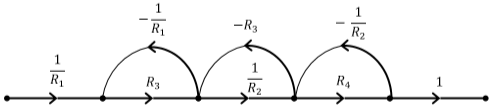
\includegraphics{flusso}
		\label{fig:flusso}
	\end{figure}
	
	\paragraph{Cammini aperti:}
	\[ P_1 = \frac{R_3 \cdot R_4}{R_1 \cdot R_2} \]
	\paragraph{Anelli singoli:}
	\[ P_{11} = - \frac{R_3}{R_1} \]
	\[ P_{21} = - \frac{R_3}{R_2} \]
	\[ P_{31} = - \frac{R_4}{R_2} \]
	\paragraph{Coppie di anelli che non si toccano:}
	\[ P_{12} = \left( - \frac{R_3}{R_1} \right) \cdot \left( - \frac{R_4}{R_2} \right) = \frac{R_3 \cdot R_4}{R_1 \cdot R_2} \]
	\paragraph{Delta:}
	\[ \Delta = 1 - \left( - \frac{R_3}{R_1} - \frac{R_3}{R_2} - \frac{R_4}{R_2} \right) + \frac{R_3 \cdot R_4}{R_1 \cdot R_2} \]
	\[ \Delta_1 = 1 \]
	\paragraph{Trasmittanza totale:}
	\[
	T = \frac{\frac{R_3 \cdot R_4}{R_1 \cdot R_2} \cdot 1}{\frac{R_1 \cdot R_2 + R_3 \cdot R_2 + R_3 \cdot R_1 + R_4 \cdot R_1 + R_3 \cdot R_4}{R_1 \cdot R_2}} = \frac{R_3 \cdot R_4}{R_1 \cdot R_2 + R_3 \cdot R_2 + R_3 \cdot R_1 + R_4 \cdot R_1 + R_3 \cdot R_4}
	\]
	\newpage
	
	
	\subsection{Diagrammi di Bode}
	
	\subsubsection{Esercizio 1}
	\paragraph{Testo:}
	tracciare i diagrammi di Bode della seguente funzione di trasferimento
	\[ G(s) = \frac{s+1}{s^4 + 2s^3 + 100s^2} = \frac{s+1}{s^2 \cdot (s^2 + 2s + 100)} \]
	
	\paragraph{Forma di Bode:}
	\[ G(j\omega) = \frac{1}{100} \cdot \frac{1}{(j\omega)^2} \cdot \frac{1+j\omega}{1 + \frac{2}{100} \cdot j\omega - \frac{\omega^2}{100}} \]
	
	\paragraph{Termine costante:}
	\[ H(j\omega)= 10^{-2} \]
	\begin{itemize}
		\item Modulo
			\[ |H(j\omega)|_{dB} = 20 \cdot log|10^{-2}| = -40 \text{ } dB \]
		\item Fase
			\[ arg(H(j\omega)) = 0 \]
	\end{itemize}
	\begin{figure}[h]
		\centering
		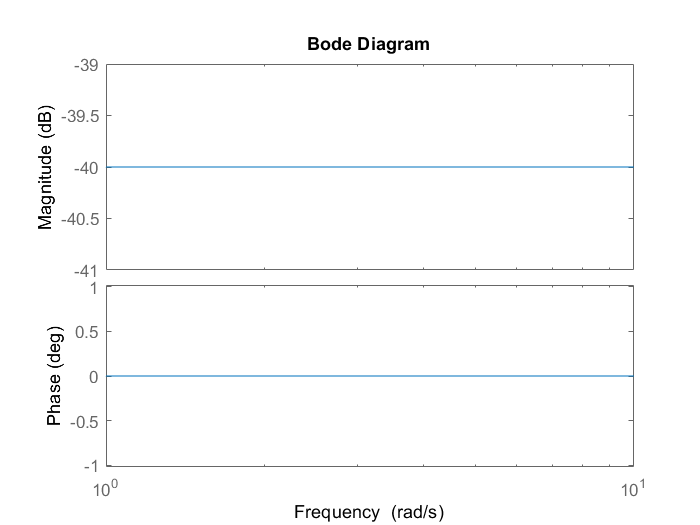
\includegraphics[scale=0.5]{costante}
		\label{fig:costante}
	\end{figure}
	
	\newpage
	\paragraph{Zeri e poli nell'origine:}
	\[ H(j\omega)=\frac{1}{(j\omega)^2} \]
	\begin{itemize}
		\item Modulo
			\[ |H(j\omega)|_{dB} = 20 \cdot (-2) \cdot log|\omega| = -40 \text{ } \frac{dB}{dec}  \]
		\item Fase
			\[ arg(H(j\omega)) = -2 \cdot 90 = -180 \]
	\end{itemize}
	\begin{figure}[h]
		\centering
		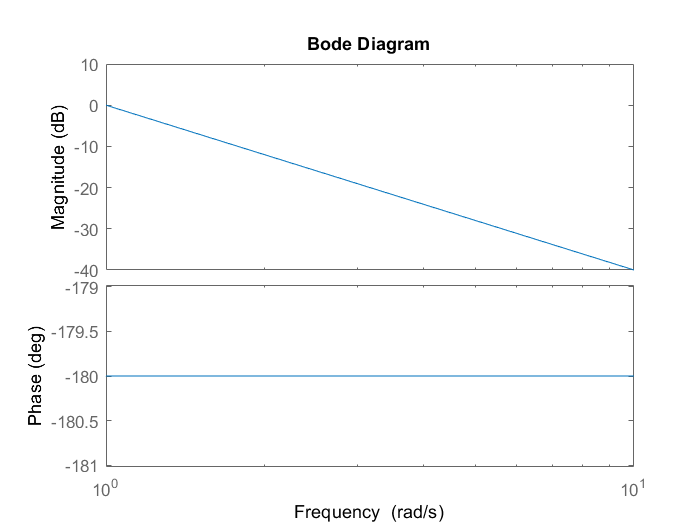
\includegraphics[scale=0.5]{origine}
		\label{fig:origine}
	\end{figure}
	
	\paragraph{Zeri e poli reali:}
	\[ \tau = 1, \text{ } \mu = 1 \]
	\[ H(j\omega)=1+j\omega \]
	\begin{itemize}
		\item Modulo
			\[
			|H(j\omega)|_{dB} =
				\begin{cases}
				0& \hspace{1.0cm} \text{se } \omega << 10^0 \\
				20 \text{ } \frac{dB}{dec}& \hspace{1.0cm} \text{se } \omega >> 10^0
				\end{cases}
			\]
		\item Fase
			\[
			arg(H(j\omega)) =
				\begin{cases}
				0& \hspace{1.0cm} \text{se } \omega << 10^0 \\
				90& \hspace{1.0cm} \text{se } \omega >> 10^0
				\end{cases}
			\]
			\paragraph{Approssimazione:}
			\[
			A = \left( 0.2, 0 \right) \text{ e } B = \left( 5, 90 \right)
			\]
	\end{itemize}
	\begin{figure}[h]
		\centering
		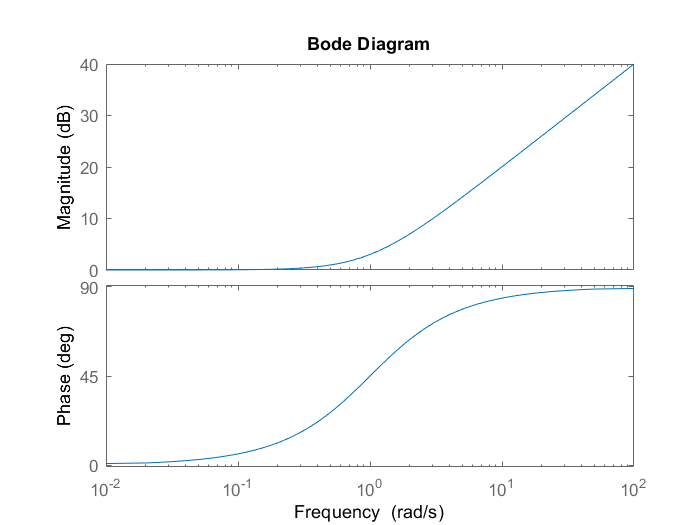
\includegraphics[scale=0.5]{reali}
		\label{fig:reali}
	\end{figure}
	\newpage
	
	\paragraph{Zeri e poli complessi coniugati:}
	\[ \omega_n=\sqrt{100}=10, \text{ } \frac{2}{10}\zeta=\frac{2}{100} \longrightarrow \zeta=\frac{1}{10}, \text{ } \mu=-1 \]
	\[ H(j\omega) = \left( 1 + \frac{2}{100} \cdot j\omega - \frac{\omega^2}{100} \right)^{-1} \]
	\begin{itemize}
		\item Modulo
			\[
			|H(j\omega)|_{dB} =
				\begin{cases}
				0& \hspace{1.0cm} \text{se } \omega << 10^1 \\
				-40 \text{ } \frac{dB}{dec}& \hspace{1.0cm} \text{se } \omega >> 10^1
				\end{cases}
			\]
		\item Fase
			\[
			arg(H(j\omega)) =
				\begin{cases}
				0& \hspace{1.0cm} \text{se } \omega << 10^1 \\
				-180& \hspace{1.0cm} \text{se } \omega >> 10^1
				\end{cases}
			\]
			\paragraph{Approssimazione:}
			\[
			A = \left( 8.5, 0 \right) \text{ e } B = \left( 11.7, -180 \right)
			\]
	\end{itemize}
	\begin{figure}[h]
		\centering
		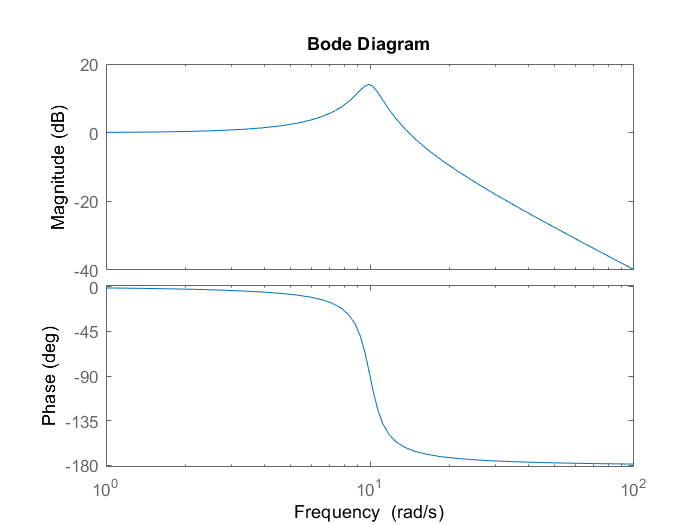
\includegraphics[scale=0.5]{complessi}
		\label{fig:complessi}
	\end{figure}
	\newpage
	
	\paragraph{Diagramma globale:}
	unendo tutti i diagrammi si ricava il seguente
	\begin{figure}[h]
		\centering
		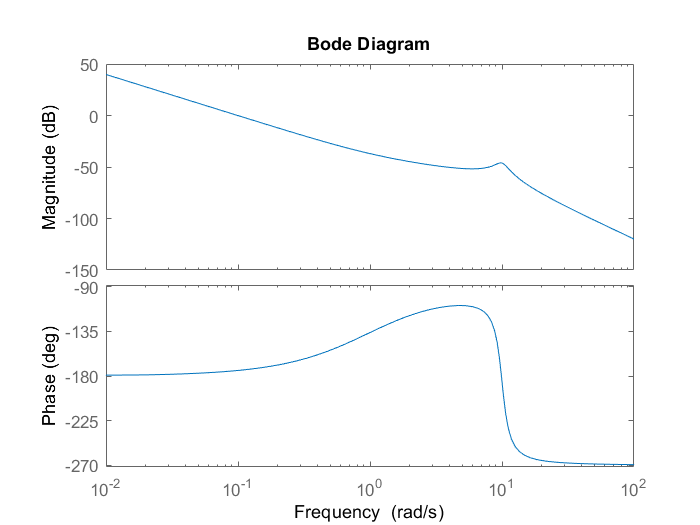
\includegraphics[scale=0.5]{globale}
		\label{fig:globale}
	\end{figure}
	\newpage
	
	
	\subsection{Sistemi LTI a tempo discreto}
	
	\subsubsection{Esercizio 1}
	\paragraph{Testo:}
	\[ v(k) + v(k-1) = u(k) - u(k-1) \]
	
	\paragraph{Stabilità asintotica:}
	\[ \left. z^0 + z^{-1} = 0 \right|_{\cdot z^n = z^1} \]
	\[ z + 1 = 0 \longrightarrow \lambda_1 = -1 \]
	Il sistema non è asintoticamente stabile perché $|\lambda_1|=1$
	
	\paragraph{BIBO stabilità:}
	\[ H(z) = \frac{z-1}{z+1} \]
	Il sistema non è BIBO stabile perché $|p_1|=1$
	
	\paragraph{Risposta impulsiva (ricorsione):}
	\[
	\begin{cases}
		v(k) = h(k) \\
		u(k) = \delta(k)
	\end{cases}
	\longrightarrow
	h(k) + h(k-1) = \delta(k) - \delta(k-1)
	\]
	\[
	k=0
	\longrightarrow
	h(0) + h(-1) = \delta(0) - \delta(-1)
	\longrightarrow
	h(0) = 1 - 0 - 0
	\longrightarrow
	h(0) = 1
	\]
	\[
	k=1
	\longrightarrow
	h(1) + h(0) = \delta(1) - \delta(0)
	\longrightarrow
	h(1) = 0 - 1 - 1
	\longrightarrow
	h(1) = -2
	\]
	\[
	k=2
	\longrightarrow
	h(2) + h(1) = \delta(2) - \delta(1)
	\longrightarrow
	h(2) = 0 - 0 + 2
	\longrightarrow
	h(2) = 2
	\]
	\[
	h(k) =
	\begin{cases}
		1& \hspace{1.0cm} \text{se } k = 0 \\
		-2& \hspace{1.0cm} \text{se } k \geq 1 \text{ e dispari} \\
		2& \hspace{1.0cm} \text{se } k \geq 1 \text{ e pari}
	\end{cases}
	\]
	\[ h(k) = d_0 \cdot \delta(k) + d_1 \cdot (-1)^k \cdot \delta_{-1}(k-1) \]
	\[
	\begin{cases}
		h(0) = d_0 \cdot \delta(0) + d_1 \cdot (-1)^0 \cdot \delta_{-1}(-1) \\
		h(1) = d_0 \cdot \delta(1) + d_1 \cdot (-1)^1 \cdot \delta_{-1}(0)
	\end{cases}
	\longrightarrow
	\begin{cases}
		d_0 = 1 \\
		- d_1 = - 2
	\end{cases}
	\longrightarrow
	\begin{cases}
		d_0 = 1 \\
		d_1 = 2
	\end{cases}
	\]
	La risposta impulsiva del sistema è $h(k) = \delta(k) + 2 \cdot (-1)^k \cdot \delta_{-1}(k-1)$
	
	\paragraph{Risposta forzata (ricorsione):}
	\[
	k=0
	\longrightarrow
	v(0) + v(-1) = u(0) - u(-1)
	\longrightarrow
	v(0) = u(0) - 0 - 0
	\longrightarrow
	v(0) = u(0)
	\]
	\[
	k=1
	\longrightarrow
	v(1) + v(0) = u(1) - u(0)
	\longrightarrow
	v(1) = u(1) - u(0) - u(0)
	\longrightarrow
	v(1) = u(1) - 2u(0)
	\]
	\[
	k=2
	\longrightarrow
	v(2) + v(1) = u(2) - u(1)
	\longrightarrow
	v(2) = u(2) - u(1) - u(1) + 2u(0)
	\longrightarrow
	v(2) = u(2) - 2u(1) + 2u(0)
	\]
	La risposta forzata del sistema è
	\[ v_f(k) = u(k) + \sum_{i=0}^{k-1} 2 \cdot (-1)^{k-i} \cdot u(i) \]

	\paragraph{Risposta forzata (convoluzione):}
	\[ h(k-i) = \delta(k-i) + 2 \cdot (-1)^{k-i} \cdot \delta_{-1}(k-i-1) \]
	\[ v_f(k) = [u*h](k) = \sum_{i=0}^k u(i) \cdot h(k-i) = \sum_{i=0}^k u(i) \cdot [\delta(k-i) + 2 \cdot (-1)^{k-i} \cdot \delta_{-1}(k-i-1)] \]
	\[ v_f(k) = [\delta(k-k) + 2 \cdot (-1)^{k-k} \cdot \delta_{-1}(k-k-1)] \cdot u(k) + \sum_{i=0}^{k-1} 2 \cdot (-1)^{k-i} \cdot u(i) \]
	\[ v_f(k) = [\delta(0) + 2 \cdot (-1)^{0} \cdot \delta_{-1}(-1)] \cdot u(k) + \sum_{i=0}^{k-1} 2 \cdot (-1)^{k-i} \cdot u(i) \]
	\[ v_f(k) = [1 + 0] \cdot u(k) + \sum_{i=0}^{k-1} 2 \cdot (-1)^{k-i} \cdot u(i) = u(k) + \sum_{i=0}^{k-1} 2 \cdot (-1)^{k-i} \cdot u(i) \]

	
	\subsubsection{Esercizio 2}
	\paragraph{Testo:}
	\[ v(k) - \frac{3}{10} v(k-1) - \frac{1}{10} v(k-2) = u(k) - \frac{2}{5} u(k-2) \]
	\[ v(-1) = 2, \text{ } v(-2) = -2, \text{ } u(k) = 2^k \cdot \delta_{-1}(k) \]

	\paragraph{Stabilità:}
	\[ \left. z^0 - \frac{3}{10} z^{-1} - \frac{1}{10} z^{-2} = 0 \right|_{\cdot z^n = z^2} \]
	\[ z^2 - \frac{3}{10} z - \frac{1}{10} = 0 \]
	\[ \lambda_{1,2} = \frac{\frac{3}{10} \pm \sqrt{\frac{9}{100} + \frac{4}{10}}}{2} = \frac{\frac{3}{10} \pm \frac{7}{10}}{2}\]
	\[ \lambda_1 = \frac{1}{2}, \text{ } \lambda_2 = - \frac{1}{5} \]
	Il sistema è asintoticamente stabile e quindi anche BIBO stabile
	
	\paragraph{Risposta libera:}
	\[ v_l(k) = c_1 \cdot \left( \frac{1}{2} \right)^k + c_2 \cdot \left( - \frac{1}{5} \right)^k \]
	\[
	\begin{cases}
		2c_1 - 5c_2 = 2 \\
		4c_1 + 25c_2 = -2
	\end{cases}
	\longrightarrow
	\begin{cases}
		c_1 = 1 + \frac{5}{2} c_2 \\
		4 + 10c_2 + 25c_2 = -2
	\end{cases}
	\longrightarrow
	\begin{cases}
		c_1 = 1 + \frac{5}{2} c_2 \\
		35c_2 = -6
	\end{cases}
	\longrightarrow
	\begin{cases}
		c_1 = \frac{4}{7} \\
		c_2 = - \frac{6}{35}
	\end{cases}
	\]
	La risposta libera del sistema è $v_l(k) = \frac{4}{7} \cdot \left( \frac{1}{2} \right)^k - \frac{6}{35} \cdot \left( - \frac{1}{5} \right)^k$
	
	\paragraph{Risposta impulsiva (fratti semplici):}
	\[ H(z) = \frac{z^2 - \frac{2}{5}}{z^2 - \frac{3}{10} z - \frac{1}{10}} = \frac{z^2 - \frac{2}{5}}{(z - \frac{1}{2})(z + \frac{1}{5})} \]
	\[ H_1(z) = \frac{H(z)}{z} = \frac{z^2 - \frac{2}{5}}{z(z - \frac{1}{2})(z + \frac{1}{5})} = \frac{A}{z} + \frac{B}{z - \frac{1}{2}} + \frac{C}{z + \frac{1}{5}} \]
	\[
	A = \left. z \cdot \frac{z^2 - \frac{2}{5}}{z(z - \frac{1}{2})(z + \frac{1}{5})} \right|_{z=0} = \left. \frac{z^2 - \frac{2}{5}}{(z - \frac{1}{2})(z + \frac{1}{5})} \right|_{z=0} = 4
	\]
	\[
	B = \left. \left( z - \frac{1}{2} \right) \cdot \frac{z^2 - \frac{2}{5}}{z(z - \frac{1}{2})(z + \frac{1}{5})} \right|_{z = \frac{1}{2}} = \left. \frac{z^2 - \frac{2}{5}}{z(z + \frac{1}{5})} \right|_{z = \frac{1}{2}} = - \frac{3}{7}
	\]
	\[
	C = \left. \left( z + \frac{1}{5} \right) \cdot \frac{z^2 - \frac{2}{5}}{z(z - \frac{1}{2})(z + \frac{1}{5})} \right|_{z = - \frac{1}{5}} = \left. \frac{z^2 - \frac{2}{5}}{z(z - \frac{1}{2})} \right|_{z = - \frac{1}{5}} = - \frac{18}{7}
	\]
	\[ H_1(z) = \frac{4}{z} - \frac{3}{7} \cdot \frac{1}{z - \frac{1}{2}} - \frac{18}{7} \cdot \frac{1}{z + \frac{1}{5}} \]
	\[ H(z) = H_1(z) \cdot z = 4 - \frac{3}{7} \cdot \frac{z}{z - \frac{1}{2}} - \frac{18}{7} \cdot \frac{z}{z + \frac{1}{5}} \]
	\[
	h(k) = \mathcal{Z} [H(z)] = 4 \cdot \delta(k) + \left[ - \frac{3}{7} \cdot \left( \frac{1}{2} \right)^k - \frac{18}{7} \cdot \left( - \frac{1}{5} \right)^k \right] \cdot \delta_{-1}(k)
	\]
	
	\paragraph{Risposta forzata (fratti semplici):}
	\[ U(z) = \mathcal{Z} \left[ 2^k \cdot \delta_{-1}(k) \right] = \frac{z}{z-2} \]
	\[ V_f(z) = H(z) \cdot U(z) = \frac{z^2 - \frac{2}{5}}{(z - \frac{1}{2})(z + \frac{1}{5})} \cdot \frac{z}{z-2} \]
	\[ V_{f_1}(z) = \frac{V_f(z)}{z} = \frac{z^2 - \frac{2}{5}}{(z - \frac{1}{2})(z + \frac{1}{5})(z-2)} = \frac{A}{z - \frac{1}{2}} + \frac{B}{z + \frac{1}{5}} + \frac{C}{z-2} \]
	\[
	A = \left. \left( z - \frac{1}{2} \right) \cdot \frac{z^2 - \frac{2}{5}}{(z - \frac{1}{2})(z + \frac{1}{5})(z-2)} \right|_{z = \frac{1}{2}} = \left. \frac{z^2 - \frac{2}{5}}{(z + \frac{1}{5})(z-2)} \right|_{z = \frac{1}{2}} = \frac{1}{7}
	\]
	\[
	B = \left. \left( z + \frac{1}{5} \right) \cdot \frac{z^2 - \frac{2}{5}}{(z - \frac{1}{2})(z + \frac{1}{5})(z-2)} \right|_{z = - \frac{1}{5}} = \left. \frac{z^2 - \frac{2}{5}}{(z - \frac{1}{2})(z-2)} \right|_{z = - \frac{1}{5}} = - \frac{18}{77}
	\]
	\[
	C = \left. \left( z - 2 \right) \cdot \frac{z^2 - \frac{2}{5}}{(z - \frac{1}{2})(z + \frac{1}{5})(z-2)} \right|_{z = 2} = \left. \frac{z^2 - \frac{2}{5}}{(z - \frac{1}{2})(z + \frac{1}{5})} \right|_{z = 2} = \frac{12}{11}
	\]
	\[ V_{f_1}(z) = \frac{1}{7} \cdot \frac{1}{z - \frac{1}{2}} - \frac{18}{77} \cdot \frac{1}{z + \frac{1}{5}} + \frac{12}{11} \cdot \frac{1}{z-2} \]
	\[ V_f(z) = V_{f_1}(z) \cdot z = \frac{1}{7} \cdot \frac{z}{z - \frac{1}{2}} - \frac{18}{77} \cdot \frac{z}{z + \frac{1}{5}} + \frac{12}{11} \cdot \frac{z}{z-2} \]
	\[
	v_f(k) = \mathcal{Z} [V_f(z)] = \left[ \frac{1}{7} \cdot \left( \frac{1}{2} \right)^k - \frac{18}{77} \cdot \left( - \frac{1}{5} \right)^k + \frac{12}{11} \cdot \left( 2 \right)^k \right] \cdot \delta_{-1}(k)
	\]
	
	
	\subsubsection{Esercizio 3}
	\paragraph{Testo:}
	\[ v(k) - v(k-1) + \frac{1}{4} v(k-2) = u(k) - 3 u(k-1) \]
	\[ v(-1) = 4, \text{ } v(-2) = 3, \text{ } u(k) = \left( -\frac{1}{2} \right)^k \cdot \delta_{-1}(k) \]
	
	\paragraph{Stabilità:}
	\[ \left. z^0 - z^{-1} + \frac{1}{4} z^{-2} = 0 \right|_{\cdot z^n = z^2} \]
	\[ z^2 - z + \frac{1}{4} = 0 \]
	\[ \lambda_{1,2} = \frac{1 \pm \sqrt{1-1}}{2} = \frac{1 \pm 0}{2} = \frac{1}{2} \]
	Il sistema è asintoticamente stabile e quindi anche BIBO stabile
	
	\paragraph{Risposta libera:}
	\[ v_l(k) = c_1 \cdot \left( \frac{1}{2} \right)^k + c_2 \cdot k \cdot \left( \frac{1}{2} \right)^k \]
	\[
	\begin{cases}
		2c_1 - 2c_2 = 4 \\
		4c_1 - 8c_2 = 3
	\end{cases}
	\longrightarrow
	\begin{cases}
		c_1 = 2 + c_2 \\
		8 + 4c_2 - 8c_2 = 3
	\end{cases}
	\longrightarrow
	\begin{cases}
		c_1 = 2 + c_2 \\
		-4c_2 = -5
	\end{cases}
	\longrightarrow
	\begin{cases}
		c_1 = \frac{13}{4} \\
		c_2 = \frac{5}{4}
	\end{cases}
	\]
	La risposta libera del sistema è $v_l(k) = \frac{13}{4} \cdot \left( \frac{1}{2} \right)^k + \frac{5}{4} \cdot k \cdot \left( \frac{1}{2} \right)^k$
	
	\paragraph{Risposta totale:}
	\[
	\left. z^0 \cdot V(z) - (z^{-1} \cdot V(z) + 4 z^0) + \frac{1}{4} \cdot (z^{-2} \cdot V(z) + 4 z^{-1} + 3 z^0) = z^0 \cdot U(z) - 3 z^{-1} \cdot U(z) \right|_{\cdot z^n = z^2}
	\]
	\[ V(z) \cdot \left( z^2 - z + \frac{1}{4} \right) -4z^2 + z + \frac{3}{4} z^2 = U(z) \cdot (z^2 - 3z) \]
	\[ V(z) = \frac{z^2 -3z}{z^2 - z + \frac{1}{4}} \cdot U(z) + \frac{\frac{13}{4} z^2 - z}{z^2 - z + \frac{1}{4}} \]
	\[
	U(z) = \mathcal{Z} \left[ \left( -\frac{1}{2} \right)^k \cdot \delta_{-1}(k) \right] = \frac{z}{z+\frac{1}{2}} 
	\longrightarrow
	V(z) = \frac{z^3 -3z^2}{(z-\frac{1}{2})^2 \cdot (z+\frac{1}{2})} + \frac{\frac{13}{4} z^2 - z}{(z-\frac{1}{2})^2}
	\]
	\[
	V(z) = \frac{z^3 -3z^2 + \frac{13}{4} z^3 - z^2 + \frac{13}{8} z^2 - \frac{1}{2} z}{(z-\frac{1}{2})^2 \cdot (z+\frac{1}{2})} 
	= \frac{\frac{17}{4} z^3 - \frac{19}{8} z^2 - \frac{1}{2} z}{(z-\frac{1}{2})^2 \cdot (z+\frac{1}{2})}
	\]
	\[
	V_1(z) = \frac{V(z)}{z} = \frac{\frac{17}{4} z^2 - \frac{19}{8} z - \frac{1}{2}}{(z-\frac{1}{2})^2 \cdot (z+\frac{1}{2})}
	= \frac{A}{z+\frac{1}{2}} + \frac{B}{z-\frac{1}{2}} + \frac{C}{(z-\frac{1}{2})^2}
	\]
	\[
	A = \left. \left( z+\frac{1}{2} \right) \cdot \frac{\frac{17}{4} z^2 - \frac{19}{8} z - \frac{1}{2}}{(z-\frac{1}{2})^2 \cdot (z+\frac{1}{2})} \right|_{z=-\frac{1}{2}} = \left. \frac{\frac{17}{4} z^2 - \frac{19}{8} z - \frac{1}{2}}{(z-\frac{1}{2})^2} \right|_{z=-\frac{1}{2}} = \frac{7}{4}
	\]
	\[
	B = \frac{d}{dz} \left. \left( \left( z-\frac{1}{2} \right)^2 \cdot \frac{\frac{17}{4} z^2 - \frac{19}{8} z - \frac{1}{2}}{(z-\frac{1}{2})^2 \cdot (z+\frac{1}{2})} \right) \right|_{z=\frac{1}{2}} = \left. \frac{\frac{17}{4} z^2 + \frac{17}{4} z - \frac{11}{16}}{(z+\frac{1}{2})^2} \right|_{z=\frac{1}{2}} = \frac{5}{2}
	\]
	\[
	C = \left. \left( z-\frac{1}{2} \right)^2 \cdot \frac{\frac{17}{4} z^2 - \frac{19}{8} z - \frac{1}{2}}{(z-\frac{1}{2})^2 \cdot (z+\frac{1}{2})} \right|_{z=\frac{1}{2}} = \left. \frac{\frac{17}{4} z^2 - \frac{19}{8} z - \frac{1}{2}}{z+\frac{1}{2}} \right|_{z=\frac{1}{2}} = -\frac{5}{8}
	\]
	\[ V_1(z) = \frac{7}{4} \cdot \frac{1}{z+\frac{1}{2}} + \frac{5}{2} \cdot \frac{1}{z-\frac{1}{2}} - \frac{5}{8} \cdot \frac{1}{(z-\frac{1}{2})^2} \]
	\[
	V(z) = V_1(z) \cdot z = \frac{7}{4} \cdot \frac{z}{z+\frac{1}{2}} + \frac{5}{2} \cdot \frac{z}{z-\frac{1}{2}} - \frac{5}{8} \cdot \frac{z}{(z-\frac{1}{2})^2}
	= \frac{7}{4} \cdot \frac{z}{z+\frac{1}{2}} + \frac{5}{2} \cdot \frac{z}{z-\frac{1}{2}} - \frac{5}{4} \cdot \frac{z \cdot \frac{1}{2}}{(z-\frac{1}{2})^2}
	\]
	\[
	v(k) = \mathcal{Z} [V(z)] = \left[ \frac{7}{4} \cdot \left( -\frac{1}{2} \right)^k + \frac{5}{2} \cdot \left( \frac{1}{2} \right)^k - \frac{5}{4} \cdot k \cdot \left( \frac{1}{2} \right)^k \right] \cdot \delta_{-1}(k)
	\]
	\newpage
	
	
	\section{Credits}
	Repository github: \url{https://github.com/zampierida98/UniVR-informatica} \\
	Indirizzo e-mail: \mail{zampieri.davide@outlook.com}
	
\end{document}